\section{Fifth axis: the $(\Eavail,W)$ deep-inelastic-tail study}
\label{sec:eavailw}

Enabling Valencia 2p2h fills about half of the low-recoil gap
(\S\ref{sec:3d-2p2h}) but leaves a separate high-$\Eavail$ data excess over
the MINERvA Tune~v1 prior, where 2p2h does not
contribute and the sub-percent pion-FSI dials cannot reach (covariance and its
qualifications: \S\ref{sec:eavailw-adopted}). Against the external generators the
high-$\Eavail$ picture is generator-dependent: GiBUU is low across the entire
tail (data/generator $1.59$ at $\Eavail\in[0.8,1.5)$ and $1.37$ at
$[1.5,3.0)$, $W$-integrated; see \S\ref{sec:eavailw-band} for GiBUU's
$E_\nu\approx\SI{20}{GeV}$ limit), whereas the GENIE CV matches the data in
$[0.8,1.5)$ and is low in $[1.5,3.0)$ (data/CV $1.09$)
(\S\ref{sec:3d-2p2h}). To test the deep-inelastic
hypothesis directly, we added the hadronic invariant mass $W$ as a fifth
OmniFold axis. The five-axis estimator is validated in \S\ref{sec:val-fiveaxis},
including a model-dependence study that establishes no bias--variance tradeoff or
new total uncertainty for this projection.

\subsection{$W$ as a fifth axis}
\label{sec:eavailw-axis}
Truth $W$ is the experimenter's invariant mass
$W=\sqrt{M^{2}+2M(E_\nu-E_\mu)-Q^{2}}$ with $M$ the struck-nucleon mass
(\texttt{CVUniverse::GetTrueExperimentersW()}); reco $W$ uses the same
calorimetric energy transfer $q_{0}$ and muon-kinematic $Q^{2}$ as the reco
$q_{3}$ estimator, with the average nucleon mass
(\texttt{CVUniverse::RecoW()}). Like $q_{3}$ --- and unlike $\Eavail$ --- $W$
is not invariant under the lateral systematic shifts, so the event loop dumps
shifted-$W$ lateral universes per universe, mirroring the $q_{3}$ treatment
(\S\ref{sec:4d}); the dump also carries truth hadronic diagnostics (proton and
pion multiplicities, leading-hadron angle). The $W$
binning $[0,1.1,1.4,1.8,2.2,3.0,100]\,\si{GeV}$ brackets the quasielastic
peak, the $\Delta$, the transition region, and the DIS tail. The five-axis
unfold $(\pT,\pPar,\Eavail,q_{3},W)$ passes the same marginalization anchors
as its predecessors: the $W$-marginal recovers the frozen 4D cross section to
\SI{\eavailMargin}{\percent} in normalization (5D/4D total $=1.0011$), with per-axis
median differences of \SIrange{0.3}{1.5}{\percent}, and the
$d\sigma/dW$ spectrum is finite and non-negative across all six bins.

\subsection{Where the excess lives in the $(\Eavail,W)$ plane}
\label{sec:eavailw-map}
Projecting the unfolded five-axis result onto $(\Eavail,W)$ and subtracting
the MINERvA Tune~v1 prediction (the analysis simulation's truth weighted by its full tune weight, i.e.\ the OmniFold prior; \emph{not} the untuned GENIE~CV of \S\ref{sec:eavailw-band}) localizes the excess
% full tune weight: \texttt{w\_truth}
(Fig.~\ref{fig:eavailWexcess}): it is \emph{predominantly deep-inelastic}.
The two highest-$\Eavail$ bands carry \SI{57}{\percent} of the positive
excess; of all positive excess, high-$\Eavail$ ($\ge\SI{0.8}{GeV}$) holds
\SI{67}{\percent}, and \SI{83}{\percent} of \emph{that} sits at
$W\ge\SI{1.8}{GeV}$, with the single largest cell the deep-DIS corner
($\Eavail>\SI{3}{GeV}$, $W>\SI{3}{GeV}$) at \SI{22}{\percent}. A secondary
low-$W$ (below \SI{1.1}{GeV}, QE-like) excess and a small $\Delta$-region
($W\simeq1.4$--$\SI{1.8}{GeV}$) deficit are also present.
This localization is a central-value statement under the nominal detector
response. The estimator seed moves these projected central values by a small
fraction of their uncertainty (\S\ref{sec:eavailw-adopted}, item~4); the shares
are ratios of differences formed from them and are not separately measured
against the seed.
The response-mismatch closure in
Appendix~\ref{app:response-mismatch} is designed to test whether an incorrect
hadronic response can move strength into or out of the low-$W$ component; it
has not yet produced a result.

\begin{figure}[H]
  \centering
  \includegraphics[width=0.85\textwidth]{excess_eavail_W}
  \caption{Unfolded data versus the MINERvA Tune~v1 prediction (GENIE~2.12.6 with the analysis tune weights, the OmniFold prior; labelled ``GENIE CV'' and ``CV'' inside the figure) across the
  % tune weights: \texttt{w\_truth}
  $(\Eavail,W)$ plane. \emph{Left:} $d\sigma/d\Eavail$ for both, integrated over
  $W$. \emph{Center:} the per-cell ratio data/CV, dimensionless, on a
  $0.5$--$1.5$ colour scale. \emph{Right:} the per-cell difference
  data\,$-$\,CV.
  \textbf{Axes are cell indices, counting from zero, on the
  $7\times6$ reporting grid}: $\Eavail$ edges
  $[0,0.1,0.2,0.4,0.8,1.5,3.0,100]\,\si{GeV}$ and $W$ edges
  $[0,1.1,1.4,1.8,2.2,3.0,100]\,\si{GeV}$, so index~6 on $\Eavail$ and
  index~5 on $W$ are wide catch bins.
  \textbf{Units and the bin-area factor:} the centre panel is a ratio of
  densities and is area-free, but the right panel is the difference of
  \emph{cell-integrated} cross sections,
  $(\mathrm{d}^{2}\sigma/\mathrm{d}\Eavail\,\mathrm{d}W)\times
  \Delta\Eavail\,\Delta W$ in \si{cm^2/nucleon}
  (App.~\ref{app:provenance}, \texttt{eavailw-excess}), so the catch-bin cells carry
  their large widths and look correspondingly bigger. Read the two panels
  together: the positive excess concentrates at high $\Eavail$ \emph{and} high
  $W$ --- the deep-inelastic region --- with a secondary low-$W$ (QE-like)
  component and a small $\Delta$-region deficit. The percentage shares quoted in
  the text are shares of the cell-integrated positive excess, i.e.\ of the right
  panel.}
  \label{fig:eavailWexcess}
\end{figure}

\subsection{Generator band: the corner against four external generators}
\label{sec:eavailw-band}
We compare the corner with spline-normalized $(\Eavail,W)$
predictions from GENIE~CV, GENIE$+$Valencia~2p2h/MEC, NuWro, and GiBUU
(Fig.~\ref{fig:eavailWband}). These are the flux-repaired predictions of
\S\ref{sec:3d-models} (App.~\ref{app:provenance}, \texttt{flux-repair}).
% rebuilt on 2026-09-27; KNOWN_ISSUES.md row 83; ledger rows VL156--VL158 supersede VL35--VL38 (App. H, pre-repair values)
The 3D and $(\Eavail,W)$ comparisons
now take each generator from one five-dimensional histogram: the in-phase-space
GENIE~CV total is \SI{2.76e-38}{cm^2/nucleon} in both. The GENIE$+$MEC
prediction uses the 3D normalization convention (App.~\ref{app:history}).
% KNOWN_ISSUES.md row 81
% The superseded provenance comment block (SUPERSEDED 2026-09-27 ... RESOLVED 2026-08-12)
% that stood here was moved verbatim to App. H, "Pre-repair values", beside
% "From \S\ref{sec:eavailw-band}, the generator inputs" (group g3 sidecar appH-additions.tex).
GENIE~CV, GENIE$+$MEC, NuWro, and GiBUU all lie below the data in the
high-$\Eavail\times$high-$W$ corner ($\Eavail\ge\SI{0.8}{GeV}$,
$W\ge\SI{1.8}{GeV}$), with data/generator $=1.14$, $1.14$, $1.16$, and $1.61$
respectively; no generator considered here reaches the data in the corner.
For GENIE and NuWro this is close to their shortfall over the
whole plane (integrated data/generator $1.11$, $1.07$ and $1.15$): the corner
ratio exceeds the integrated one by \SIrange{1}{7}{\percent} for them, against
\SI{16}{\percent} for GiBUU (integrated $1.39$; $\sigma=\SI{2.22e-38}{cm^2/nucleon}$
against the data's \SI{3.07e-38}{}). The GiBUU excess is its
event sample's energy limit: GiBUU was generated only up
% KNOWN_ISSUES.md row 82
to $E_\nu\approx\SI{20}{GeV}$ (\S\ref{sec:3d-models}), and in GENIE and NuWro neutrinos above that energy carry
\SIrange{14.3}{14.8}{\percent} of the corner cross section against
\SIrange{6.8}{7.4}{\percent} of the integrated one. Removing them from GENIE and NuWro
raises their corner-to-integrated contrast to \SIrange{9}{16}{\percent}, bracketing
GiBUU's; supplying GiBUU their share instead gives about $1.37$ in the corner against
$1.29$ integrated. On the flux-repaired predictions the corner is therefore not a
distinct deficit of any of the four generators; GiBUU is lower than the others
everywhere, and its larger corner shortfall is accounted for by its energy limit.
% Source: VALIDATION_LEDGER VL161 (docs/orchestration/state/note-capgap-20261003/); KNOWN_ISSUES 82.

Enabling Valencia 2p2h leaves the corner essentially
unchanged ($1.142\to1.139$), since 2p2h populates low $W$; it raises the
integrated prediction instead. At
$W\in[2.2,3.0)\,\si{GeV}$ the same four generators have data/generator
$=1.12$, $1.11$, $1.13$, and $1.34$, again close to their integrated ratios.
These are central-value ratios; no compatibility metric is quoted, for the
reason given in \S\ref{sec:eavailw-adopted}, item~1.

The localization of \S\ref{sec:eavailw-map} is therefore a statement relative
to the MINERvA Tune~v1 prior. Against the four external generators, the
data lie above all of them overall and in the corner.

\begin{figure}[H]
  \centering
  \includegraphics[width=0.99\textwidth]{eavailW_band}
  \caption{Unfolded $(\Eavail,W)$ cross section versus the four-generator
  band (GENIE~CV, GENIE$+$MEC, NuWro, GiBUU; GENIE and NuWro flux-repaired,
  \S\ref{sec:3d-models}). Every generator lies below the data in the high-$W$,
  high-$\Eavail$ DIS corner --- GENIE and NuWro by about their overall
  normalization shortfall, GiBUU by more; adding 2p2h leaves the corner
  unchanged because 2p2h populates low $W$.}
  \label{fig:eavailWband}
\end{figure}

Dedicated MINERvA measurements of shallow-inelastic neutrino and antineutrino
scattering also report shape and normalization disagreements with generators
\cite{MINERvA:2025sis}. They motivate tests across the resonance--DIS transition,
but their selections and reported observables differ from this inclusive
projection. They therefore provide physics context, not an independent
confirmation of the same localized excess. The location identified in the
central-value map is descriptive; a future significance must account for any
selection of the tested region using these data.
The complementary cross-check against MINERvA's published
low-recoil measurement is presented in the $(\Eavail,q_{3})$ plane
(\S\ref{sec:4d}): on the maximal common grid our central values lie
\SI{9.2}{\percent} and \SI{6.3}{\percent} above, and no covariance-based
consistency metric is reported.

\subsection{Covariance of the $(\Eavail,W)$ projection}
\label{sec:eavailw-construction}

\paragraph{Status.}
\label{sec:eavailw-adopted}
The adopted five-axis covariance is \texttt{z-cv.npz}
(\texttt{sha256}~\zcvDigest\ldots, \num{890500272} bytes, variant
\texttt{cv}), and its
$(\Eavail,W)$ projection is \texttt{sha256}~\zprojDigest\ldots\ on
\zprojCells\ cells. It is adopted under a digest-bound exception that covers
these bytes and no other candidate. Its own metadata still reads
$\texttt{scientific\_acceptance}=\text{\texttt{NON-PASSING}}$ and
$\texttt{adoptable}=\text{\texttt{false}}$, because the specification's null bound
could not be fixed before production (App.~\ref{app:release-audit}).
An earlier direct 42-bin $(\Eavail,W)$ block sum (\S\ref{sec:eavailw-cov}) is
superseded and is not quoted anywhere in this note (App.~\ref{app:history}).

\paragraph{Construction.} The adopted object projects the corrected
five-axis statistical covariance as $M C_{5D}M^{\top}$ rather than rebuilding it
in the destination binning, uses the corrected systematic endpoint convention,
and bounds the migrations omitted by the CV-support-limited dump-all sample with
selection-complete active-universe event loops. That last replacement has
landed (\S\ref{sec:uq-higherdim}). On the $\latBins$ reported cells of the
$(\pT,\pPar,\Eavail,q_{3},W)$ grid, the adopted covariance is
\begin{equation}
  \label{eq:zassembly}
  C_{Z} \;=\; D\,\Big(\textstyle\sum_{V} C_{b}\Big)\,D
  \;+\; \textstyle\sum_{R} C_{b}
  \;+\; \textstyle\sum_{A} L_{b}
  \;+\; C_{\mathrm{stat}}
  \;+\; C_{\mathrm{ML}},
\end{equation}
with the inflation $D=\diag(g)$,
\begin{equation}
  \label{eq:zinflation}
  g_{i} \;=\;
  \sqrt{\frac{\max\!\big(v^{\mathrm{cv}}_{\mathrm{uni},i},\,
                         v_{\mathrm{blk},i}\big)}
             {v_{\mathrm{blk},i}}}
  \;\ge\; 1,
  \qquad
  g_{i}\equiv 1 \ \text{ where } v_{\mathrm{blk},i}=0 .
\end{equation}
Here $v_{\mathrm{blk}}=\diag\big(\sum_{V}C_{b}\big)$ is the diagonal of the
vertical block sum and $v^{\mathrm{cv}}_{\mathrm{uni}}$ is the diagonal of the
unified-throw covariance \emph{centered on the central value}. The bins where
the denominator vanishes are pinned to $g=1$ by declaration rather than
computed; ``pinned'' and ``computed to one'' are different facts. The three band groups
$V$ (vertical), $R$ (residual) and $A$ (active lateral) are required to be
disjoint and exhaustive over the 45 bands (implementation:
App.~\ref{app:release-audit}).
Adoption was conditioned (2026-07) on documenting the low-rank treatment, mean shift, and
selection-support bound (the adopted product above) before transferring information onto a
sweep block,
$\mathbf{C}^{\syst}\!\to\!(\mathbf{C}^{\syst}-\mathbf{C}^{\mathrm{vert}})+\mathbf{G}\,\mathbf{C}^{\mathrm{vert}}\mathbf{G}$
($\mathbf{G}=\operatorname{diag}g$), which is positive-semidefinite by construction
(a direct rank-$N$ swap is not) and never falls below the block baseline.

\paragraph{Centering, explicitly.} The per-band blocks $C_{b}$ use the
MAT-conformant mean-centered $\pm1\sigma$ estimator of \S\ref{app:pair}. The
\emph{inflation operand} does not: variant \texttt{cv} takes
$v^{\mathrm{cv}}_{\mathrm{uni}}$, and the two centerings of the unified-throw
covariance differ by the outer product of the measured joint mean shift
$\mathbf{ms}$ (joint throw mean minus central value),
\begin{equation}
  \label{eq:zcentering}
  C^{\mathrm{cv}}_{\mathrm{uni}}
  = C^{\mathrm{mean}}_{\mathrm{uni}} + \mathbf{ms}\,\mathbf{ms}^{\top}
  \qquad\Longrightarrow\qquad
  v^{\mathrm{cv}}_{\mathrm{uni},i}-v^{\mathrm{mean}}_{\mathrm{uni},i}
  = \mathbf{ms}_{i}^{2},
\end{equation}
so the CV-centered variant retains the mean shift as variance where the
mean-centered variant discharges it. \textbf{That retention is the adopted
choice and is deliberate}: the mean-centered sibling measures
$\sqrt{\Tr C}$ \SI{7.13}{\percent} \emph{lower}. The variant is therefore read
from the product's own metadata and checked, never inferred from a path
(App.~\ref{app:release-audit}).

\paragraph{The projection to $(\Eavail,W)$.} The quoted 42-cell covariance is
$C_{EW}=M\,C_{Z}\,M^{\top}$ with $M$ of shape
$\zprojCells\times\latBins$ over the kept axes
$(\Eavail,W)$. Each entry of $M$ is the product of the \emph{dropped} axes'
bin widths, so the destination is a differential density in the kept axes and
carries units \si{cm^2/GeV^2/nucleon}; converting a destination cell to an
integrated cross section requires multiplying by that cell's own
$\Delta\Eavail\,\Delta W$. Its rows follow the $7\times6$ $(\Eavail,W)$ grid in
\textbf{C order}, measured rather than assumed; no source cell is dropped and the
result is exactly symmetric (App.~\ref{app:release-audit}). The support mask,
pinned mask and row-index arrays travel with the covariance and are byte-identical
between the \texttt{cv} and \texttt{mean} variants. The pairing between this covariance and
the central values shown in Fig.~\ref{fig:eavailWexcess} is established
\emph{by digest identity} --- the projected source's central-value array and the
figure's are the same bytes --- and not by numerical agreement; the numerical
agreement is a corroborating check.

\paragraph{Conditioning, and why no rank is quoted.}
The measured extremes are $\lambda_{\min}=+4.359104\times10^{-92}$ and
$\lambda_{\max}=1.488215\times10^{-77}$, so
$\lambda_{\min}/\lambda_{\max}=2.9\times10^{-15}$ and the condition number is
$\approx3.4\times10^{14}$, at the edge of double precision. There is no negative
eigenvalue, but the smallest eigenvalues sit at the floating-point noise floor of a
$\latBins$-term weighted sum, so \textbf{their sign carries no information}:
$n_{\mathrm{negative}}=0$ is a statement about this computation, not a
demonstration that the source's negative directions were cured.
The numerical rank is a property of a cutoff, not of the matrix: the 42
eigenvalues decay smoothly over about fifteen orders of magnitude with no
plateau anywhere, so the retained count is
26 at a relative cutoff $10^{-6}$, 36 at the code's default $10^{-12}$,
41 at \texttt{numpy.linalg.matrix\_rank}'s own
default $n\epsilon=9.3\times10^{-15}$, and 42 at no cutoff at all.
\textbf{A bare ``rank 36'' should not be quoted, and it is not a number of
degrees of freedom.} Any use requiring an
inverse requires a \emph{declared} regularization, which this analysis does
not supply silently (App.~\ref{app:release-audit}).

\paragraph{What the covariance supports.}
Four measurements travel with it. They are measurements, not caveats: each
bounds what may be claimed. The first, second and fourth were made on two
companion covariances built at two estimator-seed settings; only the third is a
property of these bytes.

\begin{enumerate}
\item \textbf{The estimator-seed sensitivity exceeds its declared limit.} The
  two companion covariances, at estimator-seed offsets $\{0,1200\}$, graded the
  correlation-sensitive leg at $s_{\mathrm{proj}}=\sprojMeasured\,\%$ against a
  \sprojBound\,\% movement limit fixed before production. The two
  diagonal-only legs passed ($s_{\mathrm{agg}}=\saggMeasured\,\%$,
  $s_{\mathrm{med}}=\smedMeasured\,\%$): what the failing leg sees and they do
  not is off-diagonal structure, which is precisely what a projection uses.
\item \textbf{That sensitivity is not the statistic's own resampling noise.}
  Measured with the throw ensemble held
  \emph{fixed} and only the seed changed, it does not fall with ensemble size
  over the range tested: mean $\seedEffectNforty\,\%$ over four disjoint
  40-throw subsets, $\seedEffectNeighty\,\%$ over the two 80-throw halves, and
  $\sprojMeasured\,\%$ on the full $N=160$ ensemble, giving a fitted exponent
  $\seedEffectExponent$ in $s\propto N^{-p}$. The same-seed resampling floor,
  measured at $N=40$ and $N=80$ only, falls steeply over that step ---
  $\floorNforty\,\%$ to $\floorNeighty\,\%$, a two-point exponent
  $\floorExponent$ --- and no floor measurement at $N=160$ exists. Statistical
  noise must fall with $N$; this did not fall between $N=40$ and $N=160$.
  \emph{Three limits on the reading, and they are the reason no
  infinite-ensemble statement is made here.} The $40$- and $80$-throw points are
  \emph{nested subsets} of the same 160 throws, not independent ensembles, so
  the flatness is a within-ensemble statement over a factor of four in $N$
  and the behaviour at much larger $N$ is unmeasured; the
  $\pm\seedEffectScatter\,\%$ quoted with the mean is scatter across those throw
  subsets at a \emph{single} seed pair (offsets $\{0,1200\}$), so the width of
  the seed-pair distribution is unmeasured; and the statistic is a maximum over
  the declared offset set, so further pairs can only raise it. What is
  established is that the failure of the $\sprojBound\,\%$ limit is not the
  statistic's own resampling noise, and that no reduction was observed over
  $N=40$--$160$.
\item \textbf{Five bands lie outside what the variation probes.} Five of the
  covariance's 45 bands --- the muon-energy, muon-resolution and beam-angle
  blocks --- are produced at a fixed estimator seed that the offset does not
  reach, by construction of the endpoint convention. They carry
  $\pinnedBandsSqrtTr\,\%$ of $\sqrt{\mathrm{Tr}\,C}$ and contribute exactly zero
  movement. The variation therefore does not probe their seed sensitivity, and
  what the total would show were they also to vary is unmeasured \emph{in
  either direction}: $s_{\mathrm{proj}}$ is a maximum of a relative change over
  a set of functionals, not a sum of nonnegative component contributions, so
  releasing a component that was held fixed can move the total either way.
\item \textbf{The seed also moves the central values, by a small fraction of
  their own uncertainty.} On the 43 projection functionals of the grade (these \zprojCells\ destinations plus the all-ones total rate), the central value
  moves by at most $\cvMoveProjMax\,\%$, against relative uncertainties of order
  ten percent: \textbf{at most $\cvMoveOverSigmaMax\,\%$ of the quoted
  uncertainty, median $\cvMoveOverSigmaMed\,\%$}. The largest movement falls on
  the same destination cell that drives the covariance result. Per individual
  five-axis bin it reaches $\cvMoveBinOverSigmaMax\,\%$ of that bin's
  uncertainty; the projections do not inherit that, because summing over bins
  suppresses it.
\end{enumerate}

\noindent The predeclared magnitude criterion for this estimator-seed
sensitivity remains \emph{predeclared and not computed} for this
object: it was computed only for the two companion products, built for that
purpose, and grading them does not regrade these bytes
(App.~\ref{app:provenance}, \texttt{z-adoption}).

\subsection{Validation of the five-axis estimator}
\label{sec:val-fiveaxis}
The 2D closures of \S\ref{sec:validation} do not exercise the background
subtraction: every one reweights the simulated signal and unfolds it without
background.

\subsubsection{Background subtraction and generator-sized truth changes}
\label{sec:val-negweight}

\paragraph{Background subtraction.}
End-to-end five-dimensional
pseudo-experiments that add background-simulation events and rebuild the per-bin purity
weights exactly as the measurement does return
% (scalar-5D campaign, development study D1)
the highest-$W$ column of the $(\Eavail,W)$ projection \SIrange{3.5}{4.1}{\percent} low
and the highest-$\Eavail$, highest-$W$ cell \SI{1.7}{\percent} high at nominal truth,
while the same experiments without background close to \SI{0.22}{\percent}. Set against
the quoted total uncertainty of those cells this is 0.36--1.07 standard deviations. The
bias is a property of the purity footing (\S\ref{app:negweight}), is not in any quoted
covariance, and its size on data is not established.
% Sources: docs/orchestration/OUTCOME-20260925-s5c-purity-background-bias-at-high-W.md,
% docs/orchestration/state/s5c/d1/d1_summary.json, docs/orchestration/state/s5c/d1/bias_vs_adopted.json.
With the unbinned negative-weight (\texttt{negweight-refined}) treatment
(App.~\ref{app:negweight}), sixty experiments at nominal truth bring the highest-$W$
column to \SIrange{0.11}{0.24}{\percent} and the corner cell to \SI{0.24}{\percent}.
% CLI form: \texttt{-{}-bkg-mode negweight-refined}. Implementation (refinement to
% non-negative weights before the first OmniFold step; injection and independent
% subtraction halves of the background simulation) is in App. B.
A set of joint
cells nevertheless remains \SIrange{0.7}{1.1}{\percent} high, up to 14 standard errors,
against \SI{-0.2}{\percent} without background; the mechanism is not established.
On the data, the two background treatments differ by
a median of \SI{0.36}{\percent} and at most \SI{1.4}{\percent} over the reported
functionals. This measures method sensitivity, not a bias. The negative-weight treatment
is not adopted.

\paragraph{Generator-sized truth changes.}
Experiments whose truth is reweighted by the GiBUU-to-GENIE $\Eavail$ shape ratio
(0.70--1.33 per $\Eavail$ bin, total preserved) are not followed by the unfolding. (The
ratio was built from a GENIE prediction later found to have been generated from a
mis-sampled flux, \S\ref{sec:3d-models}; it remains a valid known-truth
% KNOWN_ISSUES.md row 83
deformation of this size but is not a measured GiBUU--GENIE difference.) The
$(\Eavail,W)$ cells deviate from that truth by a median of \SI{9.7}{\percent}, up to
\SI{74}{\percent} in the highest-$W$ column, and by several percent in the largest cells.
A $q_3$ deformation that leaves the $(\Eavail,W)$ truth unchanged moves those cells by up
to \SI{37}{\percent}. Signal-only experiments with the same seeds reproduce both results,
so they are a property of the estimator (five iterations, the GBDT configuration of
\S\ref{sec:method}), not of the background treatment. This regularization
(unfolding-model) bias is in no quoted uncertainty.
% Source: docs/orchestration/OUTCOME-20260925-s5n-stage1-development-fail.md (VL151, VL152);
% KNOWN_ISSUES 75, 77; independently reproduced (state/s5n/stage1/review-round-1.md).

\subsubsection{Why the estimator does not follow a generator-sized change}
\label{sec:val-departure}
% An instrumented rerun recorded every OmniFold iteration of these experiments. It
% reproduced the development results bitwise and repeated them through the unmodified
% driver, which shows the same response to the $\Eavail$ departure (highest-$W$ cell
% \SI{73.8}{\percent} against \SI{73.5}{\percent}).
The two steps behave as intended. The first step matches the pseudo-data at reco level
within statistical noise, and the second reproduces its truth-level weight sums to
\SI{0.5}{\percent}. Yet the unfolded result folds back onto the data less well than the
true model does. On noise-free pseudo-data it reproduces more than \SI{99}{\percent} of
the departure's reco-level signal while the $(\Eavail,W)$ cells stay \SIrange{5}{11}{\percent}
off in the median and up to \SI{74}{\percent} in the worst cell. The remaining reco-level
imprint is small relative to the departure but still statistically significant at the
analysis exposure.

Thirty iterations reduce the $\Eavail$ residual by \SI{26}{\percent}, and it is still
falling slowly; the $q_3$ residual grows with iterations. A larger classifier improves the
reco-level fit without improving the $\Eavail$ truth residual, and removing the regression
for events that fail reconstruction does not help it. No single cause is established, and
no authorized estimator change passes its predeclared screen for the GiBUU-to-GENIE departure.

\paragraph{Higher-capacity background refinement and data stability.}
The residual background bias has a named cause: the refinement classifier underfits
(App.~\ref{app:negweight}).
A candidate with raised refinement capacity passes the
nominal background-inclusive closure on 40 fresh pseudo-experiments (largest deviation
2.7 standard errors) and a pooled calibration test of its statistical intervals (pull width 1.02),
which did not establish calibration for every functional.
It fails the predeclared stability test on the data: perturbing the inputs within
floating-point rounding moves the reported functionals by 0.8 statistical standard
deviations in the median and 2.6 at most; the baseline moves by the same amount (0.8 and
2.5), so this belongs to the estimator family. The same instability, at most \SI{1.2}{\percent}, explains the
difference between the driver and development pipelines on the data. A later
measurement under the same candidate found it already inside the data-bootstrap
uncertainty, which refits everything per replica: each replica carries the same rounding
spread (median \SI{0.23}{\percent} per joint cell), about \SI{37}{\percent} of the bootstrap
variance, and it is below a tenth of any total uncertainty. The central value is
reproducible only to this size.
% Source: KNOWN_ISSUES 80; docs/orchestration/RECORD-20260927-s5p-stage2-exit.md section 2 (VL155).
The later paired-bootstrap study below addresses containment for this candidate only.

\paragraph{Unfolding-model dependence.}
Under the historical shapes withheld during that assessment this unfolding-model dependence is \SIrange{2}{6}{\percent} in the median
and \SIrange{16}{31}{\percent} at most. For these other fixed generator shapes (NuWro; GENIE
with enhanced meson-exchange currents) it stays within the quoted total uncertainty in
20 of the 42 $(\Eavail,W)$ cells. Nothing is adopted.
% Source: docs/orchestration/DIAGNOSIS-20260926-s5e-oi192-estimator.md (VL153);
% docs/orchestration/OUTCOME-20260926-s5e-oi192-diagnosis-and-candidate.md (VL154); KNOWN_ISSUES 75, 77, 79, 80;
% independently reproduced (state/s5e/diag/review-round-1.md, state/s5e/cand/review-round-2.md).

\subsubsection{Model dependence, variability and reporting resolution}
\label{sec:gbdt-model-dependence}

The existing studies do not establish a bias--variance tradeoff across estimator
settings. They establish a truth-dependent response to iterations and capacity,
small repeat variability at one setting, and appreciable prior sensitivity. These
are different quantities. Evaluating them separately is also the basis of unfolding
benchmarks~\cite{Brenner2020Unfolding}; regularization bias can invalidate intervals
built from estimator variability alone~\cite{Kuusela2015Unfolding}. Neither literature
result supplies a missing variance measurement for this estimator.

The noise-free study unfolds the full simulation's reweighted reconstructed events
without background. Its baseline classifiers and missed-event regressor use 100 trees
and 8 leaves; a capacity probe uses 400 trees and 31 leaves. The repeated-experiment
study instead uses candidate $R$: five iterations, the baseline OmniFold estimators,
and a separate 400-tree, 31-leaf background-refinement classifier. Its 40 nominal
and 20 experiments at each of five departures include Poisson pseudo-data, changing
MC splits and background refinement, with estimator seed 42. These assessment
samples have since informed development and are not fresh validation here.

We integrate the same saved fine-grid outputs into 109 supported joint cells
(partition J), 27 supported coarser joint cells (H2), and 39 supported
$(\Eavail,W)$ cells (EW). Each joint partition subdivides all five axes; H2 is not
nested within J. Unsupported cells remain in the full-domain rate. The historical
interval assessment retains all 42 EW cells, including three outside the later
support rule. Definitions and normalization checks are in
App.~\ref{sec:gbdt-diagnostic-definitions}.

The truth labels describe \emph{fixed historical test deformations}: D1 is a
GiBUU/GENIE $\Eavail$ ratio; W1 a NuWro/GENIE $\Eavail$ ratio; W2 a GENIE
MEC/CV $(\Eavail,W)$ ratio; and W3 a NuWro/GENIE
$(\pT,\pPar,\Eavail)$ ratio. They predate the generator-flux repair. Removing
D1 does not make the remaining ratios corrected generator comparisons. The
$q_3$ stress changes the conditional distribution at fixed $(\Eavail,W)$ with
amplitude 0.3. None of these tests changes the simulated detector response.

\paragraph{Recovery changes, but not uniformly.}
Figure~\ref{fig:gbdt-recovery} shows the available traces, with no extension beyond
the committed iteration ranges. D1 and W1 improve slowly. For W3, the J-cell
median absolute residual is \SI{5.57}{\percent} at iteration 5 and
\SI{6.57}{\percent} at 200; the largest residual grows from
\SI{32.9}{\percent} to \SI{44.8}{\percent}. The corresponding H2 medians are
\SI{3.42}{\percent} and \SI{3.68}{\percent}. This is a persistent residual over
the measured finite scan, not a claim about infinitely many iterations or every
possible classifier. The $q_3$ stress illustrates the importance of the functional:
its EW median residual rises from \SI{4.99}{\percent} at iteration 5 to
\SI{6.42}{\percent} at 30 even while some joint-cell summaries improve.
The capacity probe changes recovery, but its affordable five-iteration setting did
not meet the frozen improvement requirement. No reporting definition qualified
under the historical usefulness and budget rules, and no measurement construction
was admitted. Those verdicts are preserved.

\begin{figure}[tbp]
\centering
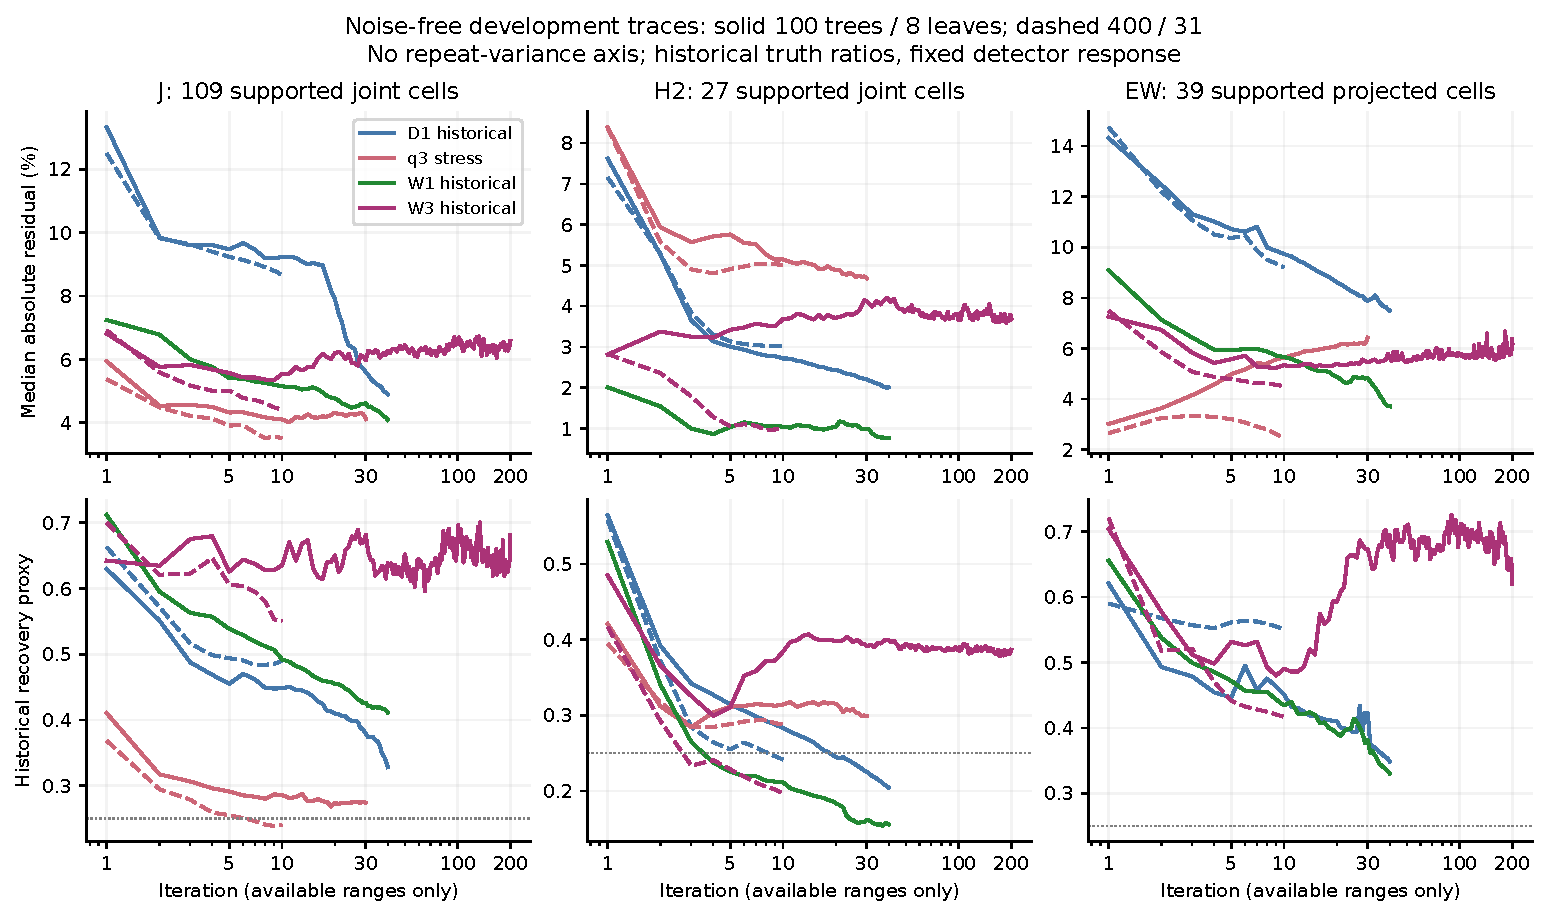
\includegraphics[width=\linewidth]{figures/gbdt_recovery.pdf}
\caption{Noise-free scalar-5D recovery for the historical test truths, at fixed
simulated response. Solid: 100 trees/8 leaves; dashed: 400/31 on the OmniFold
estimators. D1 and W1 are retained through 40 iterations, the $q_3$ stress through
30, W3 through 200, and capacity probes through 10; some baseline traces are
partial checkpoints. The upper row gives median $|\hat f/f_{\rm true}-1|$ over
supported cells. The lower row reproduces the historical proxy
$\operatorname{median}(|\hat f/f_{\rm true}-1|/|f_{\rm true}/f_0-1|)$,
restricted to departures above 1\%; the dotted line is its frozen 0.25 bound.
Its two denominators differ, so one minus this proxy is not an exact recovered
fraction. The $q_3$ stress has no eligible EW departure. No repeat variance is
measured by these traces.}
\label{fig:gbdt-recovery}
\end{figure}

\paragraph{Variability and interval behavior at five iterations.}
Figure~\ref{fig:gbdt-bias-spread} places ensemble residual means beside their
repeat standard deviations at the \emph{same} setting. At the historical W3 truth,
EW29 has a mean residual of \SI{23.67}{\percent} and repeat SD of
\SI{0.56}{\percent}; EW7 has \SI{-6.81}{\percent} and \SI{0.30}{\percent},
respectively. Small spread does not imply small bias. Coarser cells can have smaller
residuals and spread, but they estimate different integrals; this is not an improvement
in precision on an unchanged quantity. There are no matching repeat ensembles at
the longer iterations or larger OmniFold capacity from which to infer a tradeoff.

\begin{figure}[tbp]
\centering
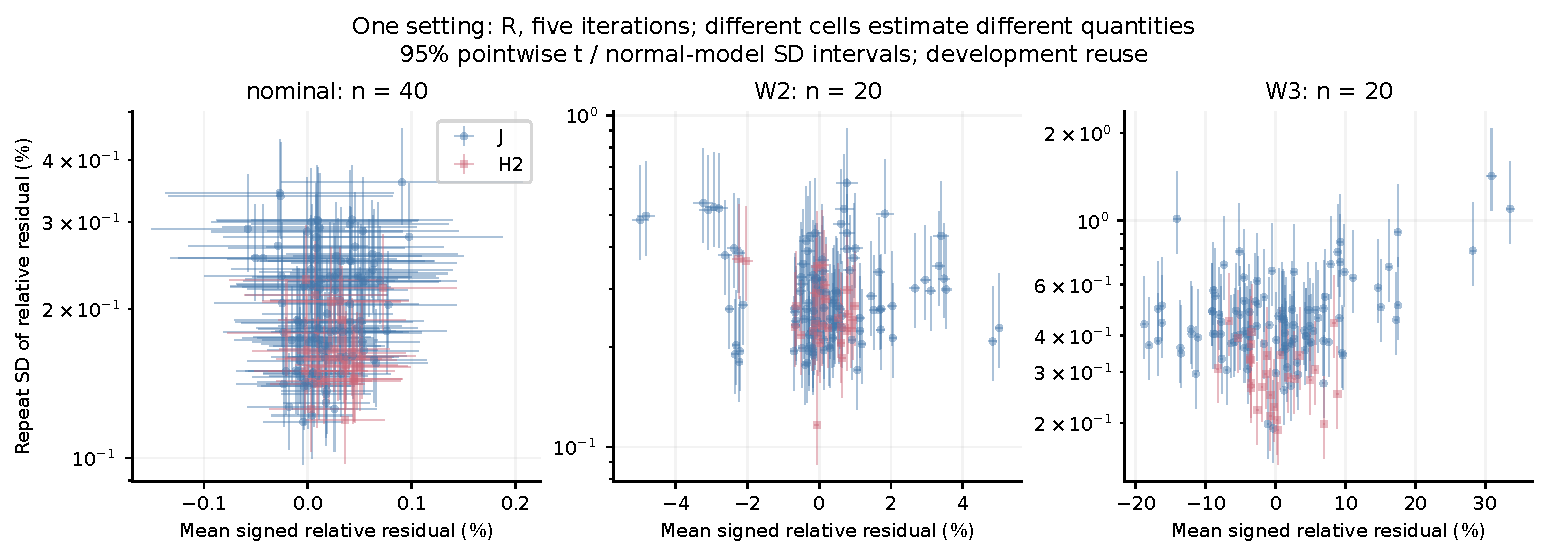
\includegraphics[width=\linewidth]{figures/gbdt_bias_spread.pdf}
\caption{Candidate $R$ at five iterations: each point is a supported J or H2 cell,
with the mean and SD of $(\hat f-f_{\rm true})/f_{\rm true}$ from the same
background-inclusive ensemble. Nominal has 40 experiments; W2 and W3 have 20
each. Bars are pointwise 95\% Student-$t$ intervals for the mean and
normal-model intervals for the SD, conditional on the saved simulation; they
are not simultaneous bounds or total uncertainties. Different truth panels and
reporting cells do not form a frontier across estimator settings.}
\label{fig:gbdt-bias-spread}
\end{figure}

The historical statistical intervals used a fixed width estimated from 100 bootstrap
replicas of \emph{one nominal development experiment}, not a width recomputed
for each assessment experiment. Their behavior is correspondingly limited
(Fig.~\ref{fig:gbdt-coverage}). For example, nominal EW41 contains the truth in
15 of 40 nominal 68\% intervals: 37.5\%, with a pointwise exact 95\% interval
of [22.7\%, 54.2\%]. A pooled calibration pass cannot qualify this cell. A later
160-experiment check using the mean of six bootstrap-width estimates changed the
pull scales, but did not validate the real-data procedure using its own width;
finite replica noise explains much of the apparent variation between those six
width estimates. Neither check establishes total coverage.

\begin{figure}[tbp]
\centering
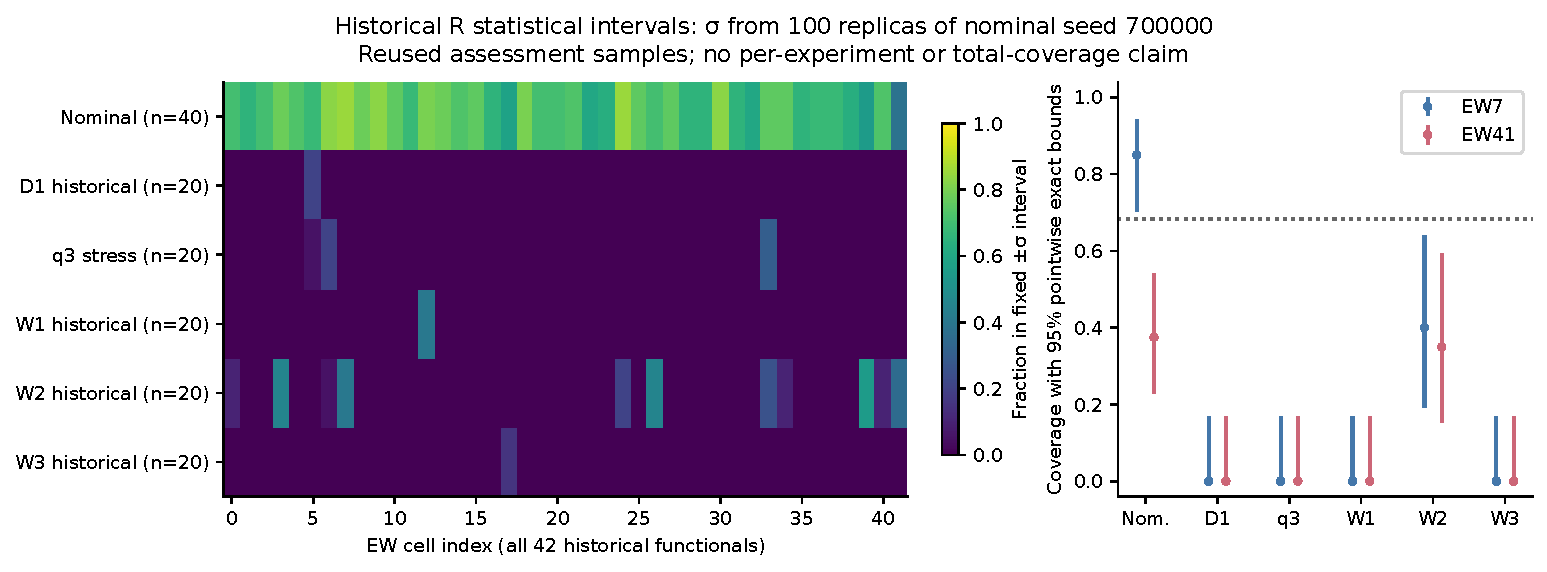
\includegraphics[width=\linewidth]{figures/gbdt_coverage.pdf}
\caption{Development reuse of the historical $R$ assessment: empirical containment
in $\hat f\pm\sigma$ with fixed nominal-bootstrap $\sigma$, on all 42 EW
functionals. The right panel shows EW7 ($\Eavail\in[0.1,0.2)$,
$W\in[1.1,1.4)$ GeV) and EW41 (both above 3 GeV), with pointwise 95\%
Clopper--Pearson bounds. The dotted line is nominal Gaussian 68.27\% coverage.
Zero of 20 contains the truth with an upper 95\% bound of 16.8\%, not zero
population coverage. Truth ratios are historical; no total-uncertainty construction
or newly validated interval is shown.}
\label{fig:gbdt-coverage}
\end{figure}

A separate paired perturbation study supports containment of rounding variability
\emph{for the tested $R$ refit-per-replica bootstrap}. Twenty edge-safe data
jitters give a J-cell median SD of \SI{0.228}{\percent}, compared with a
\SI{0.368}{\percent} bootstrap SD. Fifty bootstrap replicas with jittered partners
give a median consistency ratio of 1.02 and estimated numerical share of 0.37 of
the bootstrap variance. Adding that share again would double-count it under this
design. This does not regrade the earlier stability failure, certify interval
coverage, or transfer to the adopted covariance.

\paragraph{Prior sensitivity is not a measured real-data bias.}
Changing the prior on the real data gives shifts correlated with minus the
noise-free residual at the same historical truth (Fig.~\ref{fig:gbdt-prior}).
For W3 the correlation is 0.92 on J, yet $|\mathrm{shift}|\geq|\mathrm{residual}|$
in only 71\% of its supported cells (52\% on H2 and 54\% on EW). The maximum
shift over the five historical vertices has median 12.0\%, 9.6\% and 13.4\%
on J, H2 and EW; omitting D1 gives 11.2\%, 4.3\% and 9.9\%. These are
sensitivity envelopes, not probabilities, covariance components, or guaranteed
bias bounds. The assumption that the data truth lies within their span has not
been demonstrated.

\begin{figure}[tbp]
\centering
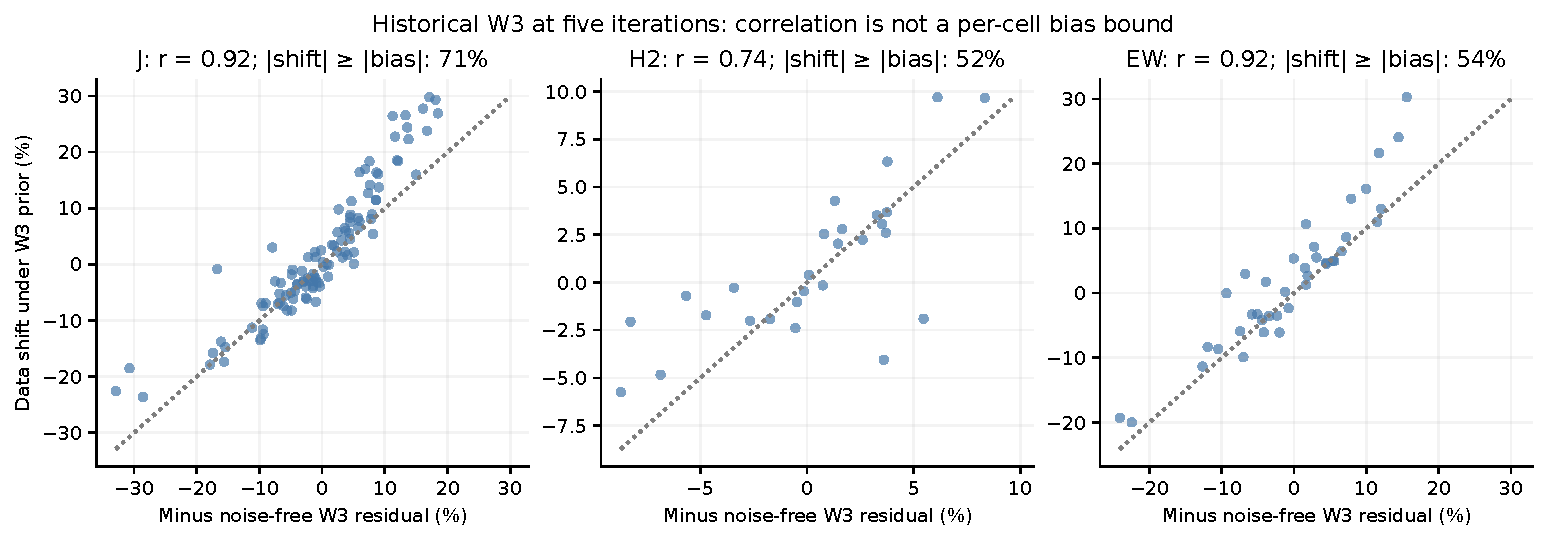
\includegraphics[width=\linewidth]{figures/gbdt_prior_response.pdf}
\caption{Historical W3 at five iterations. The horizontal quantity is minus the
noise-free relative truth residual; the vertical quantity is the relative shift
of the real-data $R$ result when its MC prior is changed to W3, normalized to the
CV-prior result. Points are supported cells, not independent repeated experiments.
The diagonal is equality. Strong correlation does not imply a per-cell bound,
and these shifts do not measure the unknown real-data bias.}
\label{fig:gbdt-prior}
\end{figure}

A decisive next measurement would use the same pseudo-data and MC splits across a
small set of iteration and capacity settings, and measure bias, variance and mean
squared error for common functionals. A statistical comparison of settings and
validation of an interval are separate tasks; total-interval validation also needs
an explicit treatment of physical nuisances and model dependence. No such new
ensemble is part of this synthesis, and the precision-measurement objective remains
unmet.
% Evidence: nd-unfolding/gbdt_model_dependence/{inputs,results,README.md}; VL163.
% Historical grades: s5e A_FAIL; s5p amendment 4 NOT ADMITTED; amendment 6 LOW corrections.

\subsubsection{Five-dimensional coverage test}
\label{sec:coverage-5d}
In five dimensions an end-to-end independent-truth test was run on the statistical
intervals of a deterministic variant of the estimator, with a nominal-truth bias
correction (1,200 pseudo-experiments over three truths). It failed its predeclared
futility criterion at the nominal and the $\Eavail$-tilted truths, so no frequentist
coverage is claimed for any five-dimensional interval.
% Source: docs/orchestration/OUTCOME-20260925-s5c-tier-s-futility-fail.md; VALIDATION_LEDGER VL150.
